\documentclass[onlymath]{beamer}
% \documentclass[onlymath,handout]{beamer}

% Macros used by all lectures, but not necessarily by excercises

%%% General setup and dependencies:

% \usetheme[ddcfooter,nosectionnum]{tud}
\usetheme[nosectionnum,pagenum,noheader]{tud}
% \usetheme[nosectionnum,pagenum]{tud}

% Increase body font size to a sane level:
\let\origframetitle\frametitle
% \renewcommand{\frametitle}[1]{\origframetitle{#1}\normalsize}
\renewcommand{\frametitle}[1]{\origframetitle{#1}\fontsize{10pt}{13.2}\selectfont}
\setbeamerfont{itemize/enumerate subbody}{size=\small} % tud defaults to scriptsize!
\setbeamerfont{itemize/enumerate subsubbody}{size=\small}
% \setbeamerfont{normal text}{size=\small}
% \setbeamerfont{itemize body}{size=\small}

\renewcommand{\emph}[1]{\textbf{#1}}

\def\arraystretch{1.3}% Make tables even less cramped vertically

\usepackage[ngerman]{babel}
\usepackage[utf8]{inputenc}
\usepackage[T1]{fontenc}

%\usepackage{graphicx}
\usepackage[export]{adjustbox} % loads graphicx
\usepackage{import}
\usepackage{stmaryrd}
\usepackage[normalem]{ulem} % sout command
% \usepackage{times}
\usepackage{txfonts}

% \usepackage[perpage]{footmisc} % reset footnote counter on each page -- fails with beamer (footnotes gone)
\usepackage{perpage}  % reset footnote counter on each page
\MakePerPage{footnote}

\usepackage{tikz}
\usetikzlibrary{arrows,positioning}
% Inspired by http://www.texample.net/tikz/examples/hand-drawn-lines/
\usetikzlibrary{decorations.pathmorphing}
\pgfdeclaredecoration{penciline}{initial}{
    \state{initial}[width=+\pgfdecoratedinputsegmentremainingdistance,
    auto corner on length=1mm,]{
        \pgfpathcurveto%
        {% From
            \pgfqpoint{\pgfdecoratedinputsegmentremainingdistance}
                      {\pgfdecorationsegmentamplitude}
        }
        {%  Control 1
        \pgfmathrand
        \pgfpointadd{\pgfqpoint{\pgfdecoratedinputsegmentremainingdistance}{0pt}}
                    {\pgfqpoint{-\pgfdecorationsegmentaspect
                     \pgfdecoratedinputsegmentremainingdistance}%
                               {\pgfmathresult\pgfdecorationsegmentamplitude}
                    }
        }
        {%TO 
        \pgfpointadd{\pgfpointdecoratedinputsegmentlast}{\pgfpoint{1pt}{1pt}}
        }
    }
    \state{final}{}
}
\tikzset{handdrawn/.style={decorate,decoration=penciline}}
\tikzset{every shadow/.style={fill=none,shadow xshift=0pt,shadow yshift=0pt}}
% \tikzset{module/.append style={top color=\col,bottom color=\col}}

% Use to make Tikz attributes with Beamer overlays
% http://tex.stackexchange.com/a/6155
\tikzset{onslide/.code args={<#1>#2}{%
  \only<#1| handout:0>{\pgfkeysalso{#2}} 
}}
\tikzset{onslideprint/.code args={<#1>#2}{%
  \only<#1>{\pgfkeysalso{#2}} 
}}

%%% Title -- always set this first

\newcommand{\defineTitle}[3]{
	\newcommand{\lectureindex}{#1}
	\title{Formale Systeme}
	\subtitle{\href{\lectureurl}{#1. Vorlesung: #2}}
	\author{\href{http://korrekt.org/}{Markus Kr\"{o}tzsch}}
%	\author{\href{http://www.sebastian-rudolph.de}{Sebastian Rudolph} in Vertretung von \href{http://korrekt.org/}{Markus Kr\"{o}tzsch}}
	\date{#3}
	\datecity{TU Dresden}
% 	\institute{Computational Logic}
}

%%% Table of contents:

\RequirePackage{ifthen}

\newcommand{\highlight}[2]{%
	\ifthenelse{\equal{#1}{\lectureindex}}{\alert{#2}}{#2}%
}

\def\myspace{-0.7ex}
\newcommand{\printtoc}{
\begin{tabular}{r@{$\quad$}l}
\highlight{1}{1.} & \highlight{1}{Willkommen/Einleitung formale Sprachen}\\[\myspace]
\highlight{2}{2.} & \highlight{2}{Grammatiken und die Chomsky-Hierarchie}\\[\myspace]
\highlight{3}{3.} & \highlight{3}{Endliche Automaten}\\[\myspace]
\highlight{4}{4.} & \highlight{4}{Complexity of FO query answering}\\[\myspace]
\highlight{5}{5.} & \highlight{5}{Conjunctive queries}\\[\myspace]
\highlight{6}{6.} & \highlight{6}{Tree-like conjunctive queries}\\[\myspace]
\highlight{7}{7.} & \highlight{7}{Query optimisation}\\[\myspace]
\highlight{8}{8.} & \highlight{8}{Conjunctive Query Optimisation / First-Order~Expressiveness}\\[\myspace]
\highlight{9}{9.} & \highlight{9}{First-Order~Expressiveness / Introduction to Datalog}\\[\myspace]
\highlight{10}{10.} & \highlight{10}{Expressive Power and Complexity of Datalog}\\[\myspace]
\highlight{11}{11.} & \highlight{11}{Optimisation and Evaluation of Datalog}\\[\myspace]
\highlight{12}{12.} & \highlight{12}{Evaluation of Datalog (2)}\\[\myspace]
\highlight{13}{13.} & \highlight{13}{Graph Databases and Path Queries}\\[\myspace]
\highlight{14}{14.} & \highlight{14}{Outlook: database theory in practice}
\end{tabular}
}

\newcommand{\overviewslide}{%
\begin{frame}\frametitle{Overview}
\printtoc
\medskip

Siehe \href{\lectureurl}{course homepage [$\Rightarrow$ link]} for more information and materials
\end{frame}
}

%%% Colours:

\usepackage{xcolor,colortbl}
\definecolor{redhighlights}{HTML}{FFAA66}
\definecolor{lightblue}{HTML}{55AAFF}
\definecolor{lightred}{HTML}{FF5522}
\definecolor{lightpurple}{HTML}{DD77BB}
\definecolor{lightgreen}{HTML}{55FF55}
\definecolor{darkred}{HTML}{CC4411}
\definecolor{darkblue}{HTML}{176FC0}%{1133AA}
\definecolor{nightblue}{HTML}{2010A0}%{1133AA}
\definecolor{alert}{HTML}{176FC0}
\definecolor{darkgreen}{HTML}{36AB14}
\definecolor{strongyellow}{HTML}{FFE219}
\definecolor{devilscss}{HTML}{666666}

\newcommand{\redalert}[1]{\textcolor{darkred}{#1}}

%%% Style commands

\newcommand{\quoted}[1]{\texttt{"}{#1}\texttt{"}}
\newcommand{\squote}{\texttt{"}} % straight quote
\newcommand{\Sterm}[1]{\ensuremath{\mathtt{\textcolor{purple}{#1}}}}    % letters in alphabets
\newcommand{\Snterm}[1]{\textsf{\textcolor{darkblue}{#1}}} % nonterminal symbols
\newcommand{\Sntermsub}[2]{\Snterm{#1}_{\Snterm{#2}}} % nonterminal symbols
\newcommand{\Slang}[1]{\textbf{\textcolor{black}{#1}}}    % languages
\newcommand{\Slangsub}[2]{\Slang{#1}_{\Slang{#2}}}    % languages
% Code
\newcommand{\Scode}[1]{\textbf{#1}}    % reserved words in program listings, e.g., "if"
\newcommand{\Scodelit}[1]{\textcolor{purple}{#1}}    % literals in program listings, e.g., strings
\newcommand{\Scomment}[1]{\textcolor{gray}{#1}}    % comment in program listings

\newcommand{\epstrastar}{\mathrel{\mathord{\stackrel{\epsilon}{\to}}{}^*}} % transitive reflexive closure of epsilon transitions in an epslion-NFA

\newcommand{\narrowcentering}[1]{\mbox{}\hfill#1\hfill\mbox{}}

\newcommand{\defeq}{\mathrel{:=}}

\newcommand{\Smach}[1]{\ensuremath{\mathcal{#1}}}    % machines

%%% Slide layout commands:

\newcommand{\sectionSlide}[1]{
\frame{\begin{center}
\LARGE
#1
\end{center}}
}
\newcommand{\sectionSlideNoHandout}[1]{
\frame<handout:0>{\begin{center}
\LARGE
#1
\end{center}}
}

\newcommand{\mydualbox}[3]{%
 \begin{minipage}[t]{#1}
 \begin{beamerboxesrounded}[upper=block title,lower=block body,shadow=true]%
    {\centering\usebeamerfont*{block title}#2}%
    \raggedright%
    \usebeamerfont{block body}
%     \small
    #3%
  \end{beamerboxesrounded}
  \end{minipage}
}
% 
\newcommand{\myheaderbox}[2]{%
 \begin{minipage}[t]{#1}
 \begin{beamerboxesrounded}[upper=block title,lower=block title,shadow=true]%
    {\centering\usebeamerfont*{block title}\rule{0pt}{2.6ex} #2}%
  \end{beamerboxesrounded}
  \end{minipage}
}

\newcommand{\mycontentbox}[2]{%
 \begin{minipage}[t]{#1}%
 \begin{beamerboxesrounded}[upper=block body,lower=block body,shadow=true]%
    {\centering\usebeamerfont*{block body}\rule{0pt}{2.6ex}#2}%
  \end{beamerboxesrounded}
  \end{minipage}
}

\newcommand{\mylcontentbox}[2]{%
 \begin{minipage}[t]{#1}%
 \begin{beamerboxesrounded}[upper=block body,lower=block body,shadow=true]%
    {\flushleft\usebeamerfont*{block body}\rule{0pt}{2.6ex}#2}%
  \end{beamerboxesrounded}
  \end{minipage}
}

% label=180:{\rotatebox{90}{{\footnotesize\textcolor{darkgreen}{Beispiel}}}}
% \hspace{-8mm}\ghost{\raisebox{-7mm}{\rotatebox{90}{{\footnotesize\textcolor{darkgreen}{Beispiel}}}}}\hspace{8mm}
\newcommand{\examplebox}[1]{%
	\begin{tikzpicture}[decoration=penciline, decorate]
		\pgfmathsetseed{1235}
		\node (n1) [decorate,draw=darkgreen, fill=darkgreen!10,thick,align=left,text width=\linewidth, inner ysep=2mm, inner xsep=2mm] at (0,0) {#1};
% 		\node (n2) [align=left,text width=\linewidth,inner sep=0mm] at (n1.92) {{\footnotesize\raisebox{3mm}{\textcolor{darkgreen}{Beispiel}}}};
% 		\node (n2) [decorate,draw=darkgreen, fill=darkgreen!10,thick, align=left,text width=\linewidth,inner sep=2mm] at (n1.90) {{\footnotesize\raisebox{0mm}{\textcolor{darkgreen}{Beispiel}}}};
	\end{tikzpicture}%
}%

\newcommand{\codebox}[1]{%
	\begin{tikzpicture}[decoration=penciline, decorate]
		\pgfmathsetseed{1236}
		\node (n1) [decorate,draw=strongyellow, fill=strongyellow!10,thick,align=left,text width=\linewidth, inner ysep=2mm, inner xsep=2mm] at (0,0) {#1};
	\end{tikzpicture}%
}%

\newcommand{\defbox}[1]{%
	\begin{tikzpicture}[decoration=penciline, decorate]
		\pgfmathsetseed{1237}
		\node (n1) [decorate,draw=darkred, fill=darkred!10,thick,align=left,text width=\linewidth, inner ysep=2mm, inner xsep=2mm] at (0,0) {#1};
	\end{tikzpicture}%
}%

\newcommand{\theobox}[1]{%
	\begin{tikzpicture}[decoration=penciline, decorate]
		\pgfmathsetseed{1240}
		\node (n1) [decorate,draw=darkblue, fill=darkblue!10,thick,align=left,text width=\linewidth, inner ysep=2mm, inner xsep=2mm] at (0,0) {#1};
	\end{tikzpicture}%
}%

\newcommand{\anybox}[2]{%
	\begin{tikzpicture}[decoration=penciline, decorate]
		\pgfmathsetseed{1240}
		\node (n1) [decorate,draw=#1, fill=#1!10,thick,align=left,text width=\linewidth, inner ysep=2mm, inner xsep=2mm] at (0,0) {#2};
	\end{tikzpicture}%
}%


\newsavebox{\mybox}%
\newcommand{\doodlebox}[2]{%
\sbox{\mybox}{#2}%
	\begin{tikzpicture}[decoration=penciline, decorate]
		\pgfmathsetseed{1238}
		\node (n1) [decorate,draw=#1, fill=#1!10,thick,align=left,inner sep=1mm] at (0,0) {\usebox{\mybox}};
	\end{tikzpicture}%
}%

% Common notation

\usepackage{amsmath,amssymb,amsfonts}
\usepackage{xspace}

\newcommand{\lectureurl}{https://iccl.inf.tu-dresden.de/web/FS2016}

\DeclareMathAlphabet{\mathsc}{OT1}{cmr}{m}{sc} % Let's have \mathsc since the slide style has no working \textsc

% Dual of "phantom": make a text that is visible but intangible
\newcommand{\ghost}[1]{\raisebox{0pt}[0pt][0pt]{\makebox[0pt][l]{#1}}}

\newcommand{\tuple}[1]{\langle{#1}\rangle}

%%% Annotation %%%

\usepackage{color}
\newcommand{\todo}[1]{{\tiny\color{red}\textbf{TODO: #1}}}



%%% Old macros below; move when needed

\newcommand{\blank}{\text{\textvisiblespace}} % empty tape cell for TM

% table syntax
\newcommand{\dom}{\textbf{dom}}
\newcommand{\adom}{\textbf{adom}}
\newcommand{\dbconst}[1]{\texttt{"#1"}}
\newcommand{\pred}[1]{\textsf{#1}}
\newcommand{\foquery}[2]{#2[#1]}
\newcommand{\ground}[1]{\textsf{ground}(#1)}
% \newcommand{\foquery}[2]{\{#1\mid #2\}} %% Notation as used in Alice Book
% \newcommand{\foquery}[2]{\tuple{#1\mid #2}}

\newcommand{\quantor}{\mathord{\reflectbox{$\text{\sf{Q}}$}}} % the generic quantor

% logic syntax
\newcommand{\Inter}{\mathcal{I}} %used to denote an interpretation
\newcommand{\Jnter}{\mathcal{J}} %used to denote another interpretation
\newcommand{\Knter}{\mathcal{K}} %used to denote yet another interpretation
\newcommand{\Zuweisung}{\mathcal{Z}} %used to denote a variable assignment

% query languages
\newcommand{\qlang}[1]{{\sf #1}} % Font for query languages
\newcommand{\qmaps}[1]{\textbf{QM}({\sf #1})} % Set of query mappings for a query language

%%% Complexities %%%

\hyphenation{Exp-Time} % prevent "Ex-PTime" (see, e.g. Tobies'01, Glimm'07 ;-)
\hyphenation{NExp-Time} % better that than something else

% \newcommand{\complclass}[1]{{\sc #1}\xspace} % font for complexity classes
\newcommand{\complclass}[1]{\ensuremath{\mathsc{#1}}\xspace} % font for complexity classes

\newcommand{\ACzero}{\complclass{AC$_0$}}
\newcommand{\LogSpace}{\complclass{L}}
\newcommand{\NLogSpace}{\complclass{NL}}
\newcommand{\PTime}{\complclass{P}}
\newcommand{\NP}{\complclass{NP}}
\newcommand{\coNP}{\complclass{coNP}}
\newcommand{\PH}{\complclass{PH}}
\newcommand{\PSpace}{\complclass{PSpace}}
\newcommand{\NPSpace}{\complclass{NPSpace}}
\newcommand{\ExpTime}{\complclass{ExpTime}}
\newcommand{\NExpTime}{\complclass{NExpTime}}
\newcommand{\ExpSpace}{\complclass{ExpSpace}}
\newcommand{\TwoExpTime}{\complclass{2ExpTime}}
\newcommand{\NTwoExpTime}{\complclass{N2ExpTime}}
\newcommand{\ThreeExpTime}{\complclass{3ExpTime}}
\newcommand{\kExpTime}[1]{\complclass{#1ExpTime}}
\newcommand{\kExpSpace}[1]{\complclass{#1ExpSpace}}


\defineTitle{6}{Reguläre Ausdrücke}{27. Oktober 2016}

\begin{document}

\maketitle

\sectionSlideNoHandout{Rückblick}

\newcommand{\myscale}{0.6}
\newcommand{\myhisymb}[1]{\boldsymbol{\textcolor{darkblue}{#1}}}

\begin{frame}\frametitle{Wiederholung: Operationen auf Automaten}

\begin{tabular}{@{\hspace{-1cm}}cr@{~~~${}={}$~~~}l}
$\myhisymb{\cup}$ & 
\scalebox{\myscale}{%
\begin{tikzpicture}[baseline={(q1.base)}]
% \draw[help lines] (0,0) grid (7,2);
\node (q1) [circle,draw=black,thick,double] at (0,0) {$A$};
\node (q2) [circle,draw=black,thick] at (2,0) {$B$};
\node (q3) [circle,draw=black,thick,double] at (4,0) {$C$};
%
\path[->,line width=0.5mm](0,0.7) edge (q1);
\path[->,line width=0.5mm](q1) edge node[above] {\Sterm{1}} (q2);
\path[->,line width=0.5mm, bend left](q2) edge node[above] {\Sterm{0}} (q3);
\path[->,line width=0.5mm, bend left](q3) edge node[above] {\Sterm{1}} (q2);
\end{tikzpicture}}
${}\myhisymb{{}\oplus{}}{}$ 
\scalebox{\myscale}{%
\begin{tikzpicture}[baseline={(p1.base)}]
% \draw[help lines] (0,0) grid (7,2);
\node (p1) [circle,draw=black,thick] at (0,0) {$D$};
\node (p2) [circle,draw=black,thick,double] at (2,0) {$E$};
%
\path[->,line width=0.5mm](0,0.7) edge (p1);
\path[->,line width=0.5mm, bend left](p1) edge node[above] {\Sterm{0}} (p2);
\path[->,line width=0.5mm, bend left](p2) edge node[above] {\Sterm{1}} (p1);
\end{tikzpicture}}
&
\scalebox{\myscale}{%
\begin{tikzpicture}[baseline={(q1.base)}]
% \draw[help lines] (0,0) grid (7,2);
\node (q1) [circle,draw=black,thick,double] at (0,0) {$A$};
\node (q2) [circle,draw=black,thick] at (2,0) {$B$};
\node (q3) [circle,draw=black,thick,double] at (4,0) {$C$};
%
\path[->,line width=0.5mm](0,0.7) edge (q1);
\path[->,line width=0.5mm](q1) edge node[above] {\Sterm{1}} (q2);
\path[->,line width=0.5mm, bend left](q2) edge node[above] {\Sterm{0}} (q3);
\path[->,line width=0.5mm, bend left](q3) edge node[above] {\Sterm{1}} (q2);
\end{tikzpicture}}
~\scalebox{\myscale}{%
\begin{tikzpicture}[baseline={(p1.base)}]
% \draw[help lines] (0,0) grid (7,2);
\node (p1) [circle,draw=black,thick] at (0,0) {$D$};
\node (p2) [circle,draw=black,thick,double] at (2,0) {$E$};
%
\path[->,line width=0.5mm](0,0.7) edge (p1);
\path[->,line width=0.5mm, bend left](p1) edge node[above] {\Sterm{0}} (p2);
\path[->,line width=0.5mm, bend left](p2) edge node[above] {\Sterm{1}} (p1);
\end{tikzpicture}}
\\[3.5ex]
%
%
$\myhisymb{\cap}$ &
\scalebox{\myscale}{\begin{tikzpicture}[baseline={(a.base)}]
% \draw[help lines] (0,0) grid (7,2);
\node (a) [circle,draw=black,thick,double] at (0,0) {$A$};
\node (b) [circle,draw=black,thick] at (3,0) {$B$};
%
\path[->,line width=0.5mm](0,1) edge (a);
\path[->,line width=0.5mm, bend left](a) edge node[above] {\Sterm{0}} (b);
\path[->,line width=0.5mm, bend left](b) edge node[above] {\Sterm{0}} (a);
\path[->,line width=0.5mm](a) edge [loop below] node[below] {\Sterm{1}} (a);
\path[->,line width=0.5mm](b) edge [loop below] node[below] {\Sterm{1}} (b);
% ,onslide={<7>{dashed,darkred}}
\end{tikzpicture}}
%
${}\myhisymb{{}\otimes{}}{}$ 
%
\scalebox{\myscale}{\begin{tikzpicture}[baseline={(current bounding box.center)}]
% \draw[help lines] (0,0) grid (7,2);
\node (c) [circle,draw=black,thick] at (0,0) {$C$};
\node (d) [circle,draw=black,thick,double] at (0,-2) {$D$};
%
\path[->,line width=0.5mm](-1,0) edge (c);
\path[->,line width=0.5mm](-1,-2) edge (d);
\path[->,line width=0.5mm](c) edge node[right] {\Sterm{0}, \Sterm{1}} (d);
\path[->,line width=0.5mm](c) edge [loop right] node[right] {\Sterm{0}} (c);
\path[->,line width=0.5mm](d) edge [loop right] node[right] {\Sterm{1}} (d);
% ,onslide={<7>{dashed,darkred}}
\end{tikzpicture}}
&
\scalebox{\myscale}{\begin{tikzpicture}[baseline={(current bounding box.center)}]
% \draw[help lines] (0,0) grid (7,2);
\node (ac) [rectangle,rounded corners=1.5ex,draw=black,thick] at (0,0) {$\tuple{A,C}$};
\node (ad) [rectangle,rounded corners=1.5ex,draw=black,thick,double] at (0,-2) {$\tuple{A,D}$};
\node (bc) [rectangle,rounded corners=1.5ex,draw=black,thick] at (3,0) {$\tuple{B,C}$};
\node (bd) [rectangle,rounded corners=1.5ex,draw=black,thick] at (3,-2) {$\tuple{B,D}$};
%
{\path[->,line width=0.5mm](-0.5,0.7) edge (ac);}
{\path[->,line width=0.5mm](-0.5,-1.3) edge (ad);}
{\path[->,line width=0.5mm, bend left](ac) edge node[below] {\Sterm{0}} (bc);}
{\path[->,line width=0.5mm, bend left](bc) edge node[above] {\Sterm{0}} (ac);}
%
{\path[->,line width=0.5mm](bc.240) edge node[below,xshift=7mm,yshift=3mm] {\Sterm{0}} (ad.35);}
{\path[->,line width=0.5mm](bc) edge node[right] {\Sterm{1}} (bd);}
{
\path[-,line width=1.1mm,white,shorten >=3mm,shorten <=3mm](ac.300) edge (bd.135);
\path[->,line width=0.5mm](ac.300) edge node[below,xshift=-7mm,yshift=3mm] {\Sterm{0}} (bd.135);
}
{\path[->,line width=0.5mm](ac) edge node[right] {\Sterm{1}} (ad);}
%
{\path[->,line width=0.5mm](bd) edge [loop right] node[right] {\Sterm{1}} (bd);}
{\path[->,line width=0.5mm](ad) edge [loop right] node[right] {\Sterm{1}} (ad);}
% ,onslide={<7>{dashed,darkred}}
\end{tikzpicture}}
\\[13mm]
%
%
$\myhisymb{\overline{\phantom{L}}}$ & 
$\overline{%
\scalebox{\myscale}{\begin{tikzpicture}[baseline={(a.base)}]
% \draw[help lines] (0,0) grid (7,2);
\node (a) [circle,draw=black,thick,double] at (0,0) {$A$};
\node (b) [circle,draw=black,thick] at (3,0) {$B$};
%
\path[->,line width=0.5mm](0,0.7) edge (a);
\path[->,line width=0.5mm, bend left](a) edge node[below] {\Sterm{0}} (b);
\path[->,line width=0.5mm, bend left](b) edge node[above] {\Sterm{0}} (a);
\path[->,line width=0.5mm](a) edge [loop left] node[left] {\Sterm{1}} (a);
\path[->,line width=0.5mm](b) edge [loop right] node[right] {\Sterm{1}} (b);
% ,onslide={<7>{dashed,darkred}}
\end{tikzpicture}}}$
&
\scalebox{\myscale}{\begin{tikzpicture}[baseline={(a.base)}]
% \draw[help lines] (0,0) grid (7,2);
\node (a) [circle,draw=black,thick] at (0,0) {$A$};
\node (b) [circle,draw=black,thick,double] at (3,0) {$B$};
%
\path[->,line width=0.5mm](0,0.7) edge (a);
\path[->,line width=0.5mm, bend left](a) edge node[below] {\Sterm{0}} (b);
\path[->,line width=0.5mm, bend left](b) edge node[above] {\Sterm{0}} (a);
\path[->,line width=0.5mm](a) edge [loop left] node[left] {\Sterm{1}} (a);
\path[->,line width=0.5mm](b) edge [loop right] node[right] {\Sterm{1}} (b);
% ,onslide={<7>{dashed,darkred}}
\end{tikzpicture}}
\\[6mm]
%
%
$\myhisymb{\circ}$ & 
\scalebox{\myscale}{%
\begin{tikzpicture}[baseline={(q1.base)}]
% \draw[help lines] (0,0) grid (7,2);
\node (q1) [circle,draw=black,thick,double] at (0,0) {$A$};
\node (q2) [circle,draw=black,thick] at (2,0) {$B$};
\node (q3) [circle,draw=black,thick,double] at (4,0) {$C$};
%
\path[->,line width=0.5mm](0,1) edge (q1);
\path[->,line width=0.5mm](q1) edge node[above] {\Sterm{1}} (q2);
\path[->,line width=0.5mm, bend left](q2) edge node[above] {\Sterm{0}} (q3);
\path[->,line width=0.5mm, bend left](q3) edge node[above] {\Sterm{1}} (q2);
\end{tikzpicture}}
${}\myhisymb{{}\odot{}}{}$ 
\scalebox{\myscale}{%
\begin{tikzpicture}[baseline={(p1.base)}]
% \draw[help lines] (0,0) grid (7,2);
\node (p1) [circle,draw=black,thick] at (0,0) {$D$};
\node (p2) [circle,draw=black,thick,double] at (2,0) {$E$};
%
\path[->,line width=0.5mm](0,1) edge (p1);
\path[->,line width=0.5mm, bend left](p1) edge node[above] {\Sterm{0}} (p2);
\path[->,line width=0.5mm, bend left](p2) edge node[above] {\Sterm{1}} (p1);
\end{tikzpicture}}
&
\scalebox{\myscale}{%
\begin{tikzpicture}[baseline={(q1.base)}]
% \draw[help lines] (0,0) grid (7,2);
\node (q1) [circle,draw=black,thick] at (0,0) {$A$};
\node (q2) [circle,draw=black,thick] at (2,0) {$B$};
\node (q3) [circle,draw=black,thick] at (4,0) {$C$};
%
\path[->,line width=0.5mm](0,1) edge (q1);
\path[->,line width=0.5mm](q1) edge node[above] {\Sterm{1}} (q2);
\path[->,line width=0.5mm, bend left](q2) edge node[below,xshift=5pt] {\Sterm{0}} (q3);
\path[->,line width=0.5mm, bend left](q3) edge node[above,xshift=-5pt] {\Sterm{1}} (q2);

% \draw[help lines] (0,0) grid (7,2);
\node (p1) [circle,draw=black,thick] at (5,0) {$D$};
\node (p2) [circle,draw=black,thick,double] at (7,0) {$E$};
%
\path[->,line width=0.5mm, bend left](p1) edge node[above] {\Sterm{0}} (p2);
\path[->,line width=0.5mm, bend left](p2) edge node[above] {\Sterm{1}} (p1);
%
\path[->,line width=0.5mm, bend left](q1) edge node[above] {$\epsilon$} (p1);
\path[->,line width=0.5mm](q3) edge node[below] {$\epsilon$} (p1);
\end{tikzpicture}}
\\[3.5ex]
%
% 
${}^{\myhisymb{*}}$ & 
$\scalebox{\myscale}{%
\begin{tikzpicture}[baseline={(q1.base)}]
% \draw[help lines] (0,0) grid (7,2);
\node (q1) [circle,draw=black,thick] at (0,0) {$A$};
\node (q2) [circle,draw=black,thick] at (2,0) {$B$};
\node (q3) [circle,draw=black,thick,double] at (4,0) {$C$};
%
\path[->,line width=0.5mm](0,0.7) edge (q1);
\path[->,line width=0.5mm](q1) edge node[above] {\Sterm{1}} (q2);
\path[->,line width=0.5mm, bend left](q2) edge node[above] {\Sterm{0}} (q3);
\path[->,line width=0.5mm, bend left](q3) edge node[above] {\Sterm{1}} (q2);
\end{tikzpicture}}^{\myhisymb{*}}$
&
\scalebox{\myscale}{%
\begin{tikzpicture}[baseline={(q1.base)}]
% \draw[help lines] (0,0) grid (7,2);
\node (q1) [circle,draw=black,thick] at (0,0) {$A$};
\node (q2) [circle,draw=black,thick] at (2,0) {$B$};
\node (q3) [circle,draw=black,thick,double] at (4,0) {$C$};
\node (qf) [circle,draw=black,thick,double] at (6,0) {$q_f$};
%
\path[->,line width=0.5mm](0,0.7) edge (q1);
\path[->,line width=0.5mm](q1) edge node[above] {\Sterm{1}} (q2);
\path[->,line width=0.5mm, bend left](q2) edge node[above] {\Sterm{0}} (q3);
\path[->,line width=0.5mm, bend left](q3) edge node[above] {\Sterm{1}} (q2);
%
\path[->,line width=0.5mm, bend left](q3) edge node[below] {$\epsilon$} (q1);
\path[->,line width=0.5mm](qf) edge [loop right] node[right] {$\epsilon$} (qf);
\end{tikzpicture}}
\\
\end{tabular}

\end{frame}

\begin{frame}\frametitle{NFAs mit Wortübergängen}

~\hfill
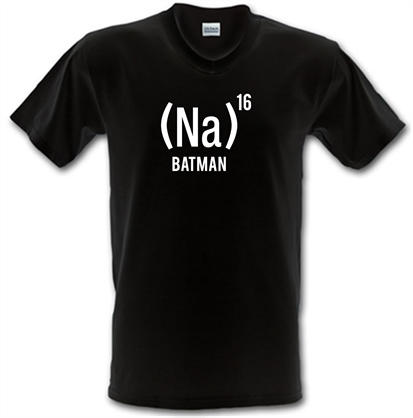
\includegraphics[height=6.5cm]{a3}
\hfill~
% \rotatebox{90}{\tiny Randall Munroe, \url{http://xkcd.com/208/}, CC-BY-NC 2.5}

\end{frame}

\begin{frame}[fragile]\frametitle{Darstellungen von Typ-3-Sprachen}

\mbox{}\hspace{-1cm}%
\begin{tikzpicture}[
	decoration=penciline, decorate,
	node distance = 7mm and 9mm,
	mybox/.style args = {#1/#2}{
		draw=#1,% line color
		fill=#2,% fill color
% 		rounded corners,
		thick,
		text width=18mm, minimum height=12mm, inner sep=1mm, 
		align=flush center
	},
	myboxlabel/.style args = {}{
		draw=devilscss,% line color
		fill=strongyellow!40,% fill color
% 		rounded corners,
		thick,
		text width=17mm, minimum height=10mm, inner sep=1.5mm, 
		align=flush center
	},
	myarrow/.style args = {#1}{
		line width=0.8mm,
		draw=#1,%line color
		%-{Triangle[length=2.8mm,width=4mm,fill=#1]},
		->,
		shorten >=0.5mm, shorten <=0.1mm
	}
]
\pgfmathsetseed{7729}
% \draw[help lines] (0,0) grid (5,5);
\node (reg) [decorate,mybox=black/cyan!40] at (2,-0.6) {reguläre Grammatik};
\node (dfa) [decorate,mybox=black/cyan!40] at (0,-4) {DFA};
\node (nfa) [decorate,mybox=black/cyan!40] at (4,-4) {NFA};
% \node (re) [decorate,mybox=black/cyan!40] at (6,-0.6) {regulärer Ausdruck};
\node (enfa) [decorate,mybox=black/cyan!40] at (8,-4) {$\epsilon$-NFA};
%
\path[myarrow=devilscss,bend left=20](dfa) edge (reg.180);
% \node (dfareglabel) [decorate,myboxlabel=,text width=19mm] at (-0.4,-0.7) {"`$q_1 \stackrel{\Sterm{a}}{\to} q_2$"' $\leadsto$ "`$q_1\to\Sterm{a}q_2$"'};
%
\path[myarrow=devilscss,-,bend left=20](reg.340) edge[->] (nfa.110);
\path[myarrow=devilscss,-,bend right=20](nfa.130) edge[->] (reg.320);
\node (regnfalabel) [decorate,myboxlabel=] at (1.6,-1.9) {\footnotesize"`$q_1\to\Sterm{a}q_2$"' $\Leftrightarrow$ "`$q_1 \stackrel{\Sterm{a}}{\to} q_2$"'};
%
\draw[myarrow=devilscss](dfa.10)--(nfa.170);
\node (dfanfalabel) [decorate,myboxlabel=,text width=16mm, minimum height=5mm,inner sep=1mm] at (1.95,-3.3) {\scalebox{0.8}{"`DFA${}\subseteq{}$NFA"'}};
%
\draw[myarrow=devilscss](nfa.190)--(dfa.350);
\node (nfadfalabel) [decorate,myboxlabel=,text width=13mm] at (2.1,-5.0) {\footnotesize Potenzm.\-konstr.};
%
\node (sd) [decorate,mybox=black/cyan!40,text width=14mm, minimum height=10mm] at (4,-6.5) {\footnotesize Syntax\-diagramm};
\draw[myarrow=devilscss,<->](sd)--(nfa);
\node (sdnfalabel) [decorate,myboxlabel=, minimum height=0mm,inner sep=1.0mm,text width=19mm] at (5.3,-5.4) {\footnotesize dualer Graph};
%%
% \path[myarrow=devilscss,-,bend left=20](nfa.70) edge[->] (re.180);
%
% \path[myarrow=devilscss,-,bend left=20,onslide={<2>{darkred}}](re.0) edge[->] (enfa);
%
\draw[myarrow=devilscss](enfa.190)--(nfa.350);
\draw[myarrow=devilscss](nfa.10)--(enfa.170);
\node (nfaenfalabel) [decorate,myboxlabel=,text width=16mm, minimum height=5mm,inner sep=1mm] at (5.95,-3.3) {\scalebox{0.75}{"`NFA${}\subseteq{}${}$\epsilon$-NFA"'}};
\node (enfanfalabel) [decorate,myboxlabel=,text width=13mm, minimum height=5mm] at (6.1,-4.6) {\footnotesize $\epsilon$-Elim.};
%
% \onslide<1>{\node (nfarelabel) [decorate,myboxlabel=,align=flush left,text width=17mm,inner sep=1mm] at (8.6,-0.7) {\footnotesize 1) komposit.\\2) explizit};}
% \onslide<2->{\node (nfarelabel) [decorate,myboxlabel=,align=flush left,text width=17mm,inner sep=1mm] at (8.6,-0.7) {\footnotesize \redalert{1) komposit.}\\2) explizit};}
%
% \node (reenfalabel) [decorate,myboxlabel=,align=flush left,text width=18mm,inner sep=1mm] at (5.6,-2.0) {\footnotesize 1) Ersetzung\\2) Dyn. Prog.};
\end{tikzpicture}

\end{frame}


\sectionSlide{Reguläre Ausdrücke}

\begin{frame}\frametitle{Endliche Sprachen}

Eine einfache Beobachtung:

\theobox{Satz: Jede endliche Sprache ist regulär.}\pause

\emph{Beweis:} Man kann eine beliebige endliche Sprache $\{w_1,\ldots, w_n\}$ durch einen
NFA mit Wortübergängen erkennen:\medskip

\narrowcentering{%
\begin{tikzpicture}[baseline={(q1.base)}]
% \draw[help lines] (0,0) grid (7,2);
\node (q1) [circle,draw=black,thick] at (0,0) {$A$};
\node (q2) [circle,draw=black,thick,double] at (4,0) {$B$};
\node (label) [draw=white] at (2,-0.1) {$\ldots$};
%
\path[->,line width=0.5mm](0,1) edge (q1);
\path[->,line width=0.5mm, bend left=45](q1) edge node[above] {$w_1$} (q2);
\path[->,line width=0.5mm, bend left=15](q1) edge node[above] {$w_2$} (q2);
\path[->,line width=0.5mm, bend right=35](q1) edge node[above] {$w_n$} (q2);
\end{tikzpicture}}\medskip

Wie in der letzten Vorlesung gezeigt, kann dieser in einen NFA umgeformt werden.
Jeder NFA akzeptiert eine reguläre Sprache.\qed

\end{frame}

\begin{frame}\frametitle{Sprachen konstruieren?}

Wir haben gesehen:\\[1ex]

\anybox{purple}{%
\vspace{-1.5ex}
\begin{itemize}%
\item Jede endliche Sprache ist regulär
\item Durch Anwendung von $\cap$, $\cup$, $\overline{\phantom{L}}$, $\circ$ und ${}^*$ entstehen aus regulären Sprachen immer wieder reguläre Sprachen.
\end{itemize}
}
\medskip

Eine natürliche Frage ist also:\\[1ex]

\anybox{strongyellow}{Welche regulären Sprachen kann man durch Anwendung von $\cap$, $\cup$, $\overline{\phantom{L}}$, $\circ$ und ${}^*$ aus endlichen Sprachen konstruieren? }
\smallskip
\pause

\narrowcentering{{\Large\redalert{Alle!}}}

\end{frame}

\begin{frame}\frametitle{Die kleinste $(\cup,\circ,{}^*)$-abgeschlossene Klasse}

Überraschender Weise sind $\cap$ und $\overline{\phantom{L}}$ nicht einmal nötig!

\theobox{Satz: Alle regulären Sprachen können durch Anwendung von $\cup$, $\circ$ und ${}^*$ aus endlichen Sprachen konstruiert werden.}

Mit $\circ$ und $\cup$ kann man jede endliche Sprache leicht aus den Sprachen $\emptyset$, $\{\epsilon\}$ und $\{\Sterm{a}\}$ ($\Sterm{a}\in\Sigma$) konstruieren.\pause
\medskip

Mit den bekannten Abschlusseigenschaften erhält man also:

\theobox{Satz: Die Klasse der regulären Sprachen ist die kleinste Klasse von Sprachen mit den folgenden Eigenschaften:
\begin{itemize}
\item Sie enthält die Sprachen $\emptyset$, $\{\epsilon\}$ und $\{\Sterm{a}\}$ für alle $\Sterm{a}\in\Sigma$
\item Sie ist abgeschlossen unter den Operatoren $\cup$, $\circ$ und ${}^*$
\end{itemize}}\pause

\emph{Beweisplan:} 
\begin{itemize}
\item Definiere diese Klasse syntaktisch: \redalert{reguläre Ausdrücke}
\item Zeige, dass diese genau die regulären Sprachen darstellen
\end{itemize}

\end{frame}

\begin{frame}\frametitle{Reguläre Ausdrücke}

% % Das bedeutet, weder $\cap$ noch $\overline{~}$ sind wirklich nötig!
% \bigskip
% 
Das motiviert die Einführung einer eigenen Syntax:

\defbox{Die Menge der \redalert{regulärer Ausdrücke} über einem Alphabet $\Sigma$ ist induktiv\footnote{D.h. die Menge der regulären Ausdrücke ist die kleinste Menge,\\ welche die Bedingungen erfüllt.} wie folgt definiert:
\begin{itemize}
\item $\emptyset$ ist ein regulärer Ausdruck
\item $\epsilon$ ist ein regulärer Ausdruck
\item $\Sterm{a}$ ist ein regulärer Ausdruck für jedes $\Sterm{a}\in\Sigma$
\item Wenn $\alpha$ und $\beta$ reguläre Ausdrücke sind,\\dann sind auch $(\alpha\beta)$, $(\alpha\mid\beta)$ und $(\alpha)^*$ reguläre Ausdrücke
\end{itemize}
}

Anmerkung: Manchmal werden $(\alpha+\beta)$ statt $(\alpha\mid\beta)$ und $(\alpha\circ\beta)$ oder $(\alpha\cdot\beta)$ statt $(\alpha\beta)$ verwendet

\examplebox{Beispiele regulärer Ausdrücke sind $(\Sterm{a}(\Sterm{b})^*)$ oder auch $((((\epsilon\mid \epsilon))^*)^*$.}

\end{frame}

\begin{frame}\frametitle{Reguläre Ausdrücke als formale Sprache}

Man kann die Menge der regulären Ausdrücke über dem Alphabet $\Sigma=\{\sigma_1, \ldots, \sigma_n\}$
auch als kontextfreie Grammatik über dem Alphabet $\Sigma\cup\{\Sterm{\emptyset},\Sterm{\epsilon},\Sterm{(},\Sterm{)},\Sterm{\mid},\Sterm{{}^*}\}$ beschreiben:
% 
\begin{align*}
 \Snterm{S} & \to \Sterm{\emptyset} \mid \Sterm{\epsilon} \mid \Snterm{A} \mid \Sterm{(}\Snterm{S}\Snterm{S}\Sterm{)} \mid \Sterm{(}\Snterm{S}\Sterm{\mid}\Snterm{S}\Sterm{)}\mid \Sterm{(}\Snterm{S}\Sterm{)}\Sterm{{}^*}\\
 \Snterm{A} & \to \sigma_1\mid \ldots \mid \sigma_n
\end{align*}\pause

Solche Notationen werden in der Praxis oft weiter vereinfacht:

\begin{itemize}
\item Endliche Mengen als Nichtterminale:
\[\Snterm{S} \to \Sterm{\emptyset} \mid \Sterm{\epsilon} \mid \Sigma \mid \Sterm{(}\Snterm{S}\Snterm{S}\Sterm{)} \mid \Sterm{(}\Snterm{S}\Sterm{\mid}\Snterm{S}\Sterm{)}\mid \Sterm{(}\Snterm{S}\Sterm{)}\Sterm{{}^*}\]
%
\item Mehrere Nichtterminale als Hinweis auf unterschiedliche Ausdrücke:
\[\alpha \to \Sterm{\emptyset} \mid \Sterm{\epsilon} \mid \Sigma \mid \Sterm{(}\alpha\beta\Sterm{)} \mid \Sterm{(}\alpha\,\Sterm{\mid}\,\beta\Sterm{)}\mid \Sterm{(}\alpha\Sterm{)}\Sterm{{}^*}\]
\end{itemize}

\end{frame}

\begin{frame}\frametitle{Semantik regulärer Ausdrücke}

Reguläre Ausdrücke beschreiben die erwarteten Sprachen:

\defbox{Die \redalert{Sprache eines regulären Ausdrucks} $\alpha$ wird mit $\Slang{L}(\alpha)$
bezeichnet und rekursiv definiert:
\begin{itemize}
\item $\Slang{L}(\emptyset)=\emptyset$
\item $\Slang{L}(\epsilon)=\{\epsilon\}$
\item $\Slang{L}(\Sterm{a})=\{\Sterm{a}\}$ für jedes $\Sterm{a}\in\Sigma$
\item $\Slang{L}((\alpha\beta))=\Slang{L}(\alpha)\circ\Slang{L}(\beta)$
\item $\Slang{L}((\alpha\mid\beta))=\Slang{L}(\alpha)\cup\Slang{L}(\beta)$
\item $\Slang{L}((\alpha)^*)=\Slang{L}(\alpha)^*$
\end{itemize}
}\medskip

\examplebox{Beispiel: $\Slang{L}(((\Sterm{ab}))^*)=(\Slang{L}((\Sterm{ab})))^*=
(\Slang{L}(\Sterm{a})\circ\Slang{L}(\Sterm{b}))^*= (\{\Sterm{a}\}\circ\{\Sterm{b}\})^* = \{\Sterm{ab}\}^*$}

\end{frame}

\begin{frame}\frametitle{Vereinfachte Klammerung}

Reguläre Ausdrücke können durch Klammerungsregeln vereinfacht werden:
\alert{${}^*$ bindet stärker als Konkatenation bindet stärker als $\mid$}
\medskip

\examplebox{
Beispiel: $\Sterm{a}\Sterm{b}^*\mid \Sterm{b}\Sterm{c}$ ist kurz für $((\Sterm{a}(\Sterm{b})^*)\mid (\Sterm{b}\Sterm{c}))$
}
\pause

Konkatenation und Alternative sind assoziativ:
\[
\Slang{L}((\alpha(\beta\gamma))) = \Slang{L}(((\alpha\beta)\gamma)) \qquad
\Slang{L}((\alpha\mid(\beta\mid\gamma))) = \Slang{L}(((\alpha\mid\beta)\mid\gamma))
\]
Daher ist es unproblematisch, dass die Klammerregeln die Reihenfolge nicht spezifizieren.

\examplebox{Beispiel: $\Sterm{101010}$ könnte für genau 42 verschiedene reguläre Ausdrücke stehen, unter anderem
für $(((((\Sterm{1}\Sterm{0})\Sterm{1})\Sterm{0})\Sterm{1})\Sterm{0})$, $((\Sterm{1}\Sterm{0})((\Sterm{1}\Sterm{0})(\Sterm{1}\Sterm{0})))$ und $(\Sterm{1}((\Sterm{0}((\Sterm{1}\Sterm{0})\Sterm{1}))\Sterm{0}))$.
% {\tiny 42 ist die größte Zahl $n$, deren Binärdarstellung genau $n$ reguläre Ausdrücke kodiert.}
}

\end{frame}

\begin{frame}\frametitle{Kurzschreibweisen für reguläre Ausdrücke}

Man kann eine Reihe von Kurzschreibweisen definieren:
\begin{itemize}
\item $\alpha^+$ ist kurz für $\alpha(\alpha)^*$ 
\item $\alpha?$ ist kurz für $(\alpha\mid\epsilon)$ 
\item $\alpha\{n,m\}$ mit $0\leq n\leq m$ ist kurz für $(\underbrace{\alpha\ldots\alpha}_{\text{$n$-mal}}\mid\ldots\mid\underbrace{\alpha\ldots\alpha}_{\text{$m$-mal}})$ 
\end{itemize}
\bigskip\pause

\anybox{gray}{%
Implementierungen regulärer Ausdrücke bieten auch Kurzformen für Alternativen einzelner Symbole ("`Character Classes"'):
\begin{itemize}
\item \texttt{.}: beliebiges Symbol, d.h. $\sigma_1\mid\ldots\mid\sigma_n$ falls $\Sigma=\{\sigma_1,\ldots,\sigma_n\}$
\item \texttt{[$\theta_1\cdots\theta_\ell$]}: beliebiges Symbol aus einer Liste, d.h. $\theta_1\mid\ldots\mid\theta_\ell$
\item \texttt{[\^{}$\theta_1\cdots\theta_\ell$]}: beliebiges Symbol \alert{nicht} aus einer Liste, d.h. $\sigma_1\mid\ldots\mid\sigma_\ell$ mit $\{\sigma_1,\ldots,\sigma_\ell\}=\Sigma\setminus\{\theta_1,\ldots,\theta_\ell\}$
\item Weitere Kurzformen für praktisch wichtige Fälle, z.B. \texttt{\textbackslash s} oder \texttt{[:blank:]} für Leerzeichen, \texttt{\textbackslash d} oder \texttt{[:digit:]} für Ziffern
\end{itemize}}

\redalert{Theoretiker meiden Kurzformen {\tiny(mehr Formen = mehr Fälle in Beweisen und Definitionen)}}

\end{frame}

\begin{frame}\frametitle{Regexps in der Praxis}

Reguläre Ausdrücke sind von großer praktischer Bedeutung
\begin{itemize}
\item Mustererkennung in Texten (Pattern Matching)
\item Lexer/Tokenizer
\item Suche nach Muster in Datenbanken
\item \ldots
\end{itemize}

Unterschiede zur reinen Lehre:
\begin{itemize}
\item \alert{Pattern Matching:} (1) spezifiziere eine Sprache (Suchwörter) und (2) finde deren Vorkommen (Matches) in einem längeren Wort (Text) $\leadsto$ Möglichkeiten zur Steuerung des zweiten Teils nötig (z.B. \emph{greedy} vs. \emph{lazy} matching)
\item \alert{Referenzen:} praktische Implementierungen erlauben es meist, Teile eines Matches im Muster wieder zu verwenden $\leadsto$ keine reguläre Sprache mehr
\item \alert{Escaping:} Unterscheidung von Steuerzeichen (Metazeichen) und Alphabetssymbolen ist praktisch aufwändig
\end{itemize}

\end{frame}

\begin{frame}\frametitle{Äquivalenz regulärer Ausdrücke}

\defbox{Zwei reguläre Ausdrücke $\alpha$ und $\beta$ sind \redalert{äquivalent},
in Symbolen $\alpha\equiv\beta$, wenn $\Slang{L}(\alpha)=\Slang{L}(\beta)$.}
\medskip

\examplebox{%
Typische Rechenregeln der Sprachoperationen gelten analog:
\begin{align*}
\alpha\mid\beta &\equiv \beta\mid\alpha
	& \epsilon\alpha &\equiv \alpha\epsilon\equiv\alpha\\
\alpha(\beta\mid\gamma) &\equiv \alpha\beta\mid\alpha\gamma
	& \emptyset\alpha &\equiv \alpha\emptyset\equiv\emptyset\\
(\beta\mid\gamma)\alpha &\equiv \beta\alpha\mid\gamma\alpha
	& \emptyset\mid\alpha &\equiv \alpha\mid\emptyset\equiv\alpha\\
\epsilon^* &\equiv \epsilon
	& \emptyset^* &\equiv\epsilon
\end{align*}}

\end{frame}

\sectionSlide{Von Regulären Ausdrücken zu Automaten}

\begin{frame}\frametitle{Zielstellung}

\emph{Behauptung:} Eine Sprache $\Slang{L}$ ist genau dann regulär, wenn es einen regulären
Ausdruck $\alpha$ gibt mit $\Slang{L}(\alpha)=\Slang{L}$.
\medskip

\emph{Beweis (Plan):} 
\begin{itemize}
\item Teilbehauptung 1: \alert{Für jeden regulären Ausdruck $\alpha$ gibt es einen NFA $\Smach{M}$, so dass  $\Slang{L}(\alpha)=\Slang{L}(\Smach{M})$}\\[1ex]
Zwei mögliche Beweismethoden:
\begin{enumerate}[(1)]
\item Kompositionelle Methode
\item Explizite Konstruktion
\end{enumerate}
\item Teilbehauptung 2: \alert{Für jeden NFA $\Smach{M}$ gibt es einen regulären Ausdruck $\alpha$, so dass  $\Slang{L}(\alpha)=\Slang{L}(\Smach{M})$}\\[1ex]
Zwei mögliche Beweismethoden:
\begin{enumerate}[(1)]
\item Ersetzungsmethode
\item Dynamische Programmierung
\end{enumerate}
\end{itemize}

\end{frame}

\begin{frame}[fragile]\frametitle{Darstellungen von Typ-3-Sprachen}

\mbox{}\hspace{-1cm}%
\begin{tikzpicture}[
	decoration=penciline, decorate,
	node distance = 7mm and 9mm,
	mybox/.style args = {#1/#2}{
		draw=#1,% line color
		fill=#2,% fill color
% 		rounded corners,
		thick,
		text width=18mm, minimum height=12mm, inner sep=1mm, 
		align=flush center
	},
	myboxlabel/.style args = {}{
		draw=devilscss,% line color
		fill=strongyellow!40,% fill color
% 		rounded corners,
		thick,
		text width=17mm, minimum height=10mm, inner sep=1.5mm, 
		align=flush center
	},
	myarrow/.style args = {#1}{
		line width=0.8mm,
		draw=#1,%line color
		%-{Triangle[length=2.8mm,width=4mm,fill=#1]},
		->,
		shorten >=0.5mm, shorten <=0.1mm
	}
]
\pgfmathsetseed{7729}
% \draw[help lines] (0,0) grid (5,5);
\node (reg) [decorate,mybox=black/cyan!40] at (2,-0.6) {reguläre Grammatik};
\node (dfa) [decorate,mybox=black/cyan!40] at (0,-4) {DFA};
\node (nfa) [decorate,mybox=black/cyan!40] at (4,-4) {NFA};
\node (re) [decorate,mybox=black/cyan!40] at (6,-0.6) {regulärer Ausdruck};
\node (enfa) [decorate,mybox=black/cyan!40] at (8,-4) {$\epsilon$-NFA};
%
\path[myarrow=devilscss,bend left=20](dfa) edge (reg.180);
% \node (dfareglabel) [decorate,myboxlabel=,text width=19mm] at (-0.4,-0.7) {"`$q_1 \stackrel{\Sterm{a}}{\to} q_2$"' $\leadsto$ "`$q_1\to\Sterm{a}q_2$"'};
%
\path[myarrow=devilscss,-,bend left=20](reg.340) edge[->] (nfa.110);
\path[myarrow=devilscss,-,bend right=20](nfa.130) edge[->] (reg.320);
\node (regnfalabel) [decorate,myboxlabel=] at (1.6,-1.9) {\footnotesize"`$q_1\to\Sterm{a}q_2$"' $\Leftrightarrow$ "`$q_1 \stackrel{\Sterm{a}}{\to} q_2$"'};
%
\draw[myarrow=devilscss](dfa.10)--(nfa.170);
\node (dfanfalabel) [decorate,myboxlabel=,text width=16mm, minimum height=5mm,inner sep=1mm] at (1.95,-3.3) {\scalebox{0.8}{"`DFA${}\subseteq{}$NFA"'}};
%
\draw[myarrow=devilscss](nfa.190)--(dfa.350);
\node (nfadfalabel) [decorate,myboxlabel=,text width=13mm] at (2.1,-5.0) {\footnotesize Potenzm.\-konstr.};
%
\node (sd) [decorate,mybox=black/cyan!40,text width=14mm, minimum height=10mm] at (4,-6.5) {\footnotesize Syntax\-diagramm};
\draw[myarrow=devilscss,<->](sd)--(nfa);
\node (sdnfalabel) [decorate,myboxlabel=, minimum height=0mm,inner sep=1.0mm,text width=19mm] at (5.3,-5.4) {\footnotesize dualer Graph};
%%
\path[myarrow=devilscss,-,bend left=20](nfa.70) edge[->] (re.180);
%
\path[myarrow=devilscss,-,bend left=20,onslide={<2>{darkred}}](re.0) edge[->] (enfa);
%
\draw[myarrow=devilscss](enfa.190)--(nfa.350);
\draw[myarrow=devilscss](nfa.10)--(enfa.170);
\node (nfaenfalabel) [decorate,myboxlabel=,text width=16mm, minimum height=5mm,inner sep=1mm] at (5.95,-3.3) {\scalebox{0.75}{"`NFA${}\subseteq{}${}$\epsilon$-NFA"'}};
\node (enfanfalabel) [decorate,myboxlabel=,text width=13mm, minimum height=5mm] at (6.1,-4.6) {\footnotesize $\epsilon$-Elim.};
%
\onslide<1>{\node (nfarelabel) [decorate,myboxlabel=,align=flush left,text width=17mm,inner sep=1mm] at (8.6,-0.7) {\footnotesize 1) komposit.\\2) explizit};}
\onslide<2->{\node (nfarelabel) [decorate,myboxlabel=,align=flush left,text width=17mm,inner sep=1mm] at (8.6,-0.7) {\footnotesize \redalert{1) komposit.}\\2) explizit};}
%
\node (reenfalabel) [decorate,myboxlabel=,align=flush left,text width=18mm,inner sep=1mm] at (5.6,-2.0) {\footnotesize 1) Ersetzung\\2) Dyn. Prog.};
\end{tikzpicture}

\end{frame}


\begin{frame}\frametitle{Rekursive Komposition von $\epsilon$-NFA}

Die Struktur regulärer Ausdrücke kann mit Operationen auf Automaten direkt abgebildet werden.
\medskip\pause

\alert{Für einen Ausdruck $\alpha$ definieren wir rekursiv den $\epsilon$-NFA $\Smach{M}(\alpha)$:}
\medskip

\emph{Grundfälle:}
\begin{itemize}
\item Wenn $\alpha=\emptyset$ dann $\Smach{M}(\alpha)={}$ \scalebox{1}{%
\begin{tikzpicture}[baseline={(q1.base)}]
% \draw[help lines] (0,0) grid (7,2);
\node (q1) [circle,draw=black,thick] at (0,0) {$A$};
%
\path[->,line width=0.5mm](-0.7,0) edge (q1);
\end{tikzpicture}}
%
\item Wenn $\alpha=\epsilon$ dann $\Smach{M}(\alpha)={}$ \scalebox{1}{%
\begin{tikzpicture}[baseline={(q1.base)}]
% \draw[help lines] (0,0) grid (7,2);
\node (q1) [circle,draw=black,thick, double] at (0,0) {$A$};
%
\path[->,line width=0.5mm](-0.7,0) edge (q1);
\end{tikzpicture}}
\item Wenn $\alpha=\Sterm{a}$ dann $\Smach{M}(\alpha)={}$ \scalebox{1}{%
\begin{tikzpicture}[baseline={(q1.base)}]
% \draw[help lines] (0,0) grid (7,2);
\node (q1) [circle,draw=black,thick] at (0,0) {$A$};
\node (q2) [circle,draw=black,thick,double] at (2,0) {$B$};
%
\path[->,line width=0.5mm](-0.7,0) edge (q1);
\path[->,line width=0.5mm](q1) edge node[above] {\Sterm{a}} (q2);
\end{tikzpicture}}
\end{itemize}\pause

\emph{Rekursive Fälle:}
Wir bezeichnen mit \redalert{$\textsf{elim}_\epsilon(\Smach{M})$} den NFA, der aus einem $\epsilon$-NFA $\Smach{M}$ durch Eliminierung der $\epsilon$-Übergänge entsteht.
\begin{itemize}
\item Wenn $\alpha=(\beta\gamma)$ dann $\Smach{M}(\alpha)=\textsf{elim}_\epsilon(\Smach{M}(\beta)\odot\Smach{M}(\gamma))$
\item Wenn $\alpha=(\beta\mid\gamma)$ dann $\Smach{M}(\alpha)=\Smach{M}(\beta)\oplus\Smach{M}(\gamma)$
\item Wenn $\alpha=(\beta)^*$ dann $\Smach{M}(\alpha)=\textsf{elim}_\epsilon(\Smach{M}(\beta)^*)$
\end{itemize}

\end{frame}


\begin{frame}\frametitle{Beispiel}

Regulärer Ausdruck: $\Sterm{a}\mid \Sterm{b}\Sterm{a}^*$
\bigskip

\narrowcentering{%
\begin{tikzpicture}[baseline={(q1.base)}]
\onslide<2->{\draw[dotted] (-0.8,-0.7) rectangle node[above,yshift=-0.75cm,xshift=-1.5cm] {$\Sterm{a}$}(2.5,0.7);}
\onslide<3->{\draw[dotted] (-0.8,-2.7) rectangle node[above,yshift=-0.75cm,xshift=-1.5cm] {$\Sterm{b}$}(2.5,-1.3);}
\onslide<4->{\draw[dotted] (3.2,-2.7) rectangle node[above,yshift=-0.75cm,xshift=-1.5cm] {$\Sterm{a}$}(6.5,-1.3);}
\onslide<5->{\draw[dotted] (3.0,-4.7) rectangle node[above,yshift=-1.85cm,xshift=-1.6cm] {$\Sterm{a}^*$}(6.7,-1.0);}
\onslide<6->{\draw[dotted] (-1.0,-5.3) rectangle node[above,yshift=-2.25cm,xshift=-3.6cm] {$\Sterm{b}\Sterm{a}^*$}(6.9,-0.8);}
\onslide<7->{\draw[dotted] (-1.2,-5.8) rectangle node[above,yshift=-3.45cm,xshift=-3.6cm] {$\Sterm{a}\mid \Sterm{b}\Sterm{a}^*$}(7.2,1.0);}
%
\onslide<2->{
\node (a1) [circle,draw=black,thick] at (0,0) {$1$};
\node (a2) [circle,draw=black,thick,double] at (2,0) {$2$};
\path[->,line width=0.5mm](-0.7,0) edge (a1);
\path[->,line width=0.5mm](a1) edge node[above] {\Sterm{a}} (a2);
}
%
\onslide<4->{
\node (a12) [circle,draw=black,thick] at (4,-2) {$5$};
\node (a22) [circle,draw=black,thick,double] at (6,-2) {$6$};
\onslide<-5>{\path[->,line width=0.5mm](3.3,-2) edge (a12);}
\path[->,line width=0.5mm](a12) edge node[above] {\Sterm{a}} (a22);
}
%
\onslide<5->{
\node (af2) [circle,draw=black,thick,double] at (4,-4) {$q_f$};
\onslide<-5>{\path[->,line width=0.5mm](3.3,-4) edge (af2);}
\path[->,line width=0.5mm,bend right=75,onslideprint={<7->{dashed,gray}}](a22) edge node[below] {$\epsilon$} (a12);
}
%
\onslide<3->{
\node (b1) [circle,draw=black,thick] at (0,-2) {$3$};
\node (b2) [circle,draw=black,thick,onslide={<-5>{double}}] at (2,-2) {$4$};
\path[->,line width=0.5mm](-0.7,-2) edge (b1);
\path[->,line width=0.5mm](b1) edge node[above] {\Sterm{b}} (b2);
}
%
\onslide<6->{
\path[->,line width=0.5mm,onslideprint={<7->{dashed,gray}}](b2) edge node[above] {$\epsilon$} (a12);
\path[->,line width=0.5mm,onslideprint={<7->{dashed,gray}}](b2) edge node[above] {$\epsilon$} (af2);
}
%
\onslide<7->{
\path[->,line width=0.5mm,bend left](b1) edge node[above] {\Sterm{b}} (a12);
\path[->,line width=0.5mm,bend right](b1) edge node[below] {\Sterm{b}} (af2);
\path[->,line width=0.5mm](a12) edge [loop below] node[below] {\Sterm{a}} (a12);
\node (cross1) at (3,-2) {\Huge$\textcolor{darkred}{\boldsymbol{\times}}$};
\node (cross2) at (3,-3) {\Huge$\textcolor{darkred}{\boldsymbol{\times}}$};
\node (cross2) at (5,-1.3) {\Huge$\textcolor{darkred}{\boldsymbol{\times}}$};
}
\end{tikzpicture}}

\end{frame}


\begin{frame}\frametitle{Korrektheit der Kompositionsmethode}

\theobox{Satz: Für jeden regulären Ausdruck $\alpha$ gilt $\Slang{L}(\alpha)=\Slang{L}(\Smach{M}(\alpha))$.}
\pause

\emph{Beweis:} Die Gleichheit folgt aus der Definition von $\Slang{L}(\alpha)$ und der Korrektheit der Operationen auf Automaten und der $\epsilon$-Eliminierung.\pause
\medskip

Formal ist der Beweis eine \alert{strukturelle Induktion}: wir konstruieren unsere Argumentation entlang der Struktur regulärer Ausdrücke.\pause
\begin{itemize}
\item \alert{Induktionsanfang:} Für die Grundfälle $\alpha=\emptyset$, $\alpha=\epsilon$ und $\alpha=\Sterm{a}$ ist die Behauptung leicht zu sehen\pause
\item \alert{Induktionshypothese (IH):} Die Behauptung wurde bereits für $\beta$ und $\gamma$ gezeigt, d.h. $\Slang{L}(\beta)=\Slang{L}(\Smach{M}(\beta))$ und $\Slang{L}(\gamma)=\Slang{L}(\Smach{M}(\gamma))$\pause
\item \alert{Induktionsschritt:} Im Fall $\alpha=(\beta\gamma)$ gilt:
% 
\begin{align*}
	\Slang{L}(\alpha) &\stackrel{\text{Def.}}{=}\Slang{L}(\beta)\circ\Slang{L}(\gamma)\stackrel{\text{IH}}{=}\Slang{L}(\Smach{M}(\beta))\circ\Slang{L}(\Smach{M}(\gamma))\\
	& \stackrel{\text{(1)}}{=} \Slang{L}(\Smach{M}(\beta)\odot\Smach{M}(\gamma))\stackrel{\text{(2)}}{=}\Slang{L}(\textsf{elim}_\epsilon(\Smach{M}(\beta)\odot\Smach{M}(\gamma)))\stackrel{\text{Def.}}{=}\Slang{L}(\Smach{M}(\alpha)).\\[-0.5ex]
	& ~~~~~\scalebox{0.8}{(1) Korrektheit der Operation $\odot$; (2) Korrektheit der $\epsilon$-Eliminierung}
\end{align*}%\vspace{-6mm}
% 
% 	\mbox{}\hfill{\scalebox{0.8}{(1) Korrektheit der Operation $\odot$; (2) Korrektheit der $\epsilon$-Eliminierung}}\\[0.7ex]\pause
Die Fälle $\alpha=(\beta\mid\gamma)$ und $\alpha=(\beta)^*$ sind analog.\qed
\end{itemize}

\end{frame}

% \begin{frame}\frametitle{Größe des komponierten NFA}
% 
% TODO
% 
% \end{frame}


\begin{frame}[fragile]\frametitle{Darstellungen von Typ-3-Sprachen}

\mbox{}\hspace{-1cm}%
\begin{tikzpicture}[
	decoration=penciline, decorate,
	node distance = 7mm and 9mm,
	mybox/.style args = {#1/#2}{
		draw=#1,% line color
		fill=#2,% fill color
% 		rounded corners,
		thick,
		text width=18mm, minimum height=12mm, inner sep=1mm, 
		align=flush center
	},
	myboxlabel/.style args = {}{
		draw=devilscss,% line color
		fill=strongyellow!40,% fill color
% 		rounded corners,
		thick,
		text width=17mm, minimum height=10mm, inner sep=1.5mm, 
		align=flush center
	},
	myarrow/.style args = {#1}{
		line width=0.8mm,
		draw=#1,%line color
		%-{Triangle[length=2.8mm,width=4mm,fill=#1]},
		->,
		shorten >=0.5mm, shorten <=0.1mm
	}
]
\pgfmathsetseed{7729}
% \draw[help lines] (0,0) grid (5,5);
\node (reg) [decorate,mybox=black/cyan!40] at (2,-0.6) {reguläre Grammatik};
\node (dfa) [decorate,mybox=black/cyan!40] at (0,-4) {DFA};
\node (nfa) [decorate,mybox=black/cyan!40] at (4,-4) {NFA};
\node (re) [decorate,mybox=black/cyan!40] at (6,-0.6) {regulärer Ausdruck};
\node (enfa) [decorate,mybox=black/cyan!40] at (8,-4) {$\epsilon$-NFA};
%
\path[myarrow=devilscss,bend left=20](dfa) edge (reg.180);
% \node (dfareglabel) [decorate,myboxlabel=,text width=19mm] at (-0.4,-0.7) {"`$q_1 \stackrel{\Sterm{a}}{\to} q_2$"' $\leadsto$ "`$q_1\to\Sterm{a}q_2$"'};
%
\path[myarrow=devilscss,-,bend left=20](reg.340) edge[->] (nfa.110);
\path[myarrow=devilscss,-,bend right=20](nfa.130) edge[->] (reg.320);
\node (regnfalabel) [decorate,myboxlabel=] at (1.6,-1.9) {\footnotesize"`$q_1\to\Sterm{a}q_2$"' $\Leftrightarrow$ "`$q_1 \stackrel{\Sterm{a}}{\to} q_2$"'};
%
\draw[myarrow=devilscss](dfa.10)--(nfa.170);
\node (dfanfalabel) [decorate,myboxlabel=,text width=16mm, minimum height=5mm,inner sep=1mm] at (1.95,-3.3) {\scalebox{0.8}{"`DFA${}\subseteq{}$NFA"'}};
%
\draw[myarrow=devilscss](nfa.190)--(dfa.350);
\node (nfadfalabel) [decorate,myboxlabel=,text width=13mm] at (2.1,-5.0) {\footnotesize Potenzm.\-konstr.};
%
\node (sd) [decorate,mybox=black/cyan!40,text width=14mm, minimum height=10mm] at (4,-6.5) {\footnotesize Syntax\-diagramm};
\draw[myarrow=devilscss,<->](sd)--(nfa);
\node (sdnfalabel) [decorate,myboxlabel=, minimum height=0mm,inner sep=1.0mm,text width=19mm] at (5.3,-5.4) {\footnotesize dualer Graph};
%%
\path[myarrow=devilscss,-,bend left=20](nfa.70) edge[->] (re.180);
%
\path[myarrow=devilscss,-,bend left=20,onslide={<2>{darkred}}](re.0) edge[->] (enfa);
%
\draw[myarrow=devilscss](enfa.190)--(nfa.350);
\draw[myarrow=devilscss](nfa.10)--(enfa.170);
\node (nfaenfalabel) [decorate,myboxlabel=,text width=16mm, minimum height=5mm,inner sep=1mm] at (5.95,-3.3) {\scalebox{0.75}{"`NFA${}\subseteq{}${}$\epsilon$-NFA"'}};
\node (enfanfalabel) [decorate,myboxlabel=,text width=13mm, minimum height=5mm] at (6.1,-4.6) {\footnotesize $\epsilon$-Elim.};
%
\node (nfarelabel) [decorate,myboxlabel=,align=flush left,text width=17mm,inner sep=1mm] at (8.6,-0.7) {\footnotesize 1) komposit.\\2) explizit};
\node (nfarelabel) [decorate,myboxlabel=,align=flush left,text width=17mm,inner sep=1mm] at (8.6,-0.7) {\footnotesize 1) komposit.\\\redalert{2) explizit}};
%
\node (reenfalabel) [decorate,myboxlabel=,align=flush left,text width=18mm,inner sep=1mm] at (5.6,-2.0) {\footnotesize 1) Ersetzung\\2) Dyn. Prog.};
\end{tikzpicture}

\end{frame}

\begin{frame}\frametitle{Explizite Konstruktion des NFA}
% 
% \redalert{An dieser Stelle wird die Konstruktion erklärt, bei der man von einem NFA ausgeht, dessen Kanten mit regulären Ausdrücken beschriftet sind und diese dann schrittweise zerlegt.}

\emph{Idee:}
\begin{itemize}
\item Beginne mit einem "`NFA mit RegExp-Übergängen"', bei dem Kanten mit regulären Ausdrücken beschriftet sind
\item Eliminiere diese Übergänge schrittweise, ähnlich wie beim Eliminieren von Wortübergängen
\end{itemize}
\bigskip

Es ist einfacher, das für reguläre Ausdrücke zu tun, die kein $\emptyset$ enthalten

\end{frame}


\begin{frame}\frametitle{Eliminierung von $\emptyset$}

Der folgende einfache Algorithmus erzeugt reguläre Ausdrücke ohne innere Vorkommen von $\emptyset$:\medskip

\codebox{
\emph{Eingabe:} regulärer Ausdruck $\alpha$\\
\emph{Ausgabe:} äquivalenter regulärer Ausdruck $\beta$ ohne $\emptyset$\\(falls $\Slang{L}(\alpha)\neq \emptyset$) oder $\emptyset$ (falls $\Slang{L}(\alpha)= \emptyset$)\\[1ex]

Wende die folgenden Ersetzungsregeln erschöpfend auf Teilausdrücke von $\alpha$ an:
\begin{itemize}
\item $(\gamma\mid\emptyset) \mapsto \gamma$ und $(\emptyset\mid\gamma) \mapsto \gamma$ 
\item $(\gamma\emptyset) \mapsto \emptyset$ und $(\emptyset\gamma) \mapsto \emptyset$
\item $(\emptyset)^* \mapsto \epsilon$
\end{itemize}
Gib das Ergebnis dieser Ersetzungen aus.
}\medskip

Die Korrektheit des Algorithmus folgt aus der Korrektheit der angewendeten Ersetzungsregeln

\end{frame}

\begin{frame}\frametitle{Explizite Konstruktion von NFAs}

Für den Ausdruck $\emptyset$ können wir einen NFA direkt angeben (wie vorn); andernfalls gehen wir wie folgt vor:
\bigskip

\emph{Gegeben:} regulärer Ausdruck $\alpha$ ohne $\emptyset$\pause
\medskip

Initialisierung: $\Smach{M}_{\alpha}={}$ \scalebox{1}{%
\begin{tikzpicture}[baseline={(q1.base)}]
% \draw[help lines] (0,0) grid (7,2);
\node (q1) [circle,draw=black,thick] at (0,0) {$A$};
\node (q2) [circle,draw=black,thick,double] at (2,0) {$B$};
%
\path[->,line width=0.5mm](-0.7,0) edge (q1);
\path[->,line width=0.5mm](q1) edge node[above] {$\alpha$} (q2);
\end{tikzpicture}}\\[1ex]

Solange es in $\Smach{M}_{\alpha}$ Übergänge $q\stackrel{\beta}{\to}p$ gibt, die mit einem Ausdruck $\beta\notin \{\epsilon\}\cup\Sigma$ beschriftet sind, wende eine der 
folgenden Regeln an:\pause
%
\begin{itemize}
\item  Ersetze \begin{tikzpicture}[baseline={(q1.base)}]
% \draw[help lines] (0,0) grid (7,2);
\node (q1) [circle,draw=black,thick] at (0,0) {$q$};
\node (q2) [circle,draw=black,thick,double] at (1.5,0) {$p$};
%
\path[->,line width=0.5mm](-0.7,0) edge (q1);
\path[->,line width=0.5mm](q1) edge node[above] {$(\gamma_1\gamma_2)$} (q2);
\end{tikzpicture}
durch 
\begin{tikzpicture}[baseline={(q1.base)}]
% \draw[help lines] (0,0) grid (7,2);
\node (q1) [circle,draw=black,thick] at (0,0) {$q$};
\node (r) [circle,draw=black,thick,double] at (1.5,0) {$r$};
\node (q2) [circle,draw=black,thick,double] at (3,0) {$p$};
%
\path[->,line width=0.5mm](-0.7,0) edge (q1);
\path[->,line width=0.5mm](q1) edge node[above] {$\gamma_1$} (r);
\path[->,line width=0.5mm](r) edge node[above] {$\gamma_2$} (q2);
\end{tikzpicture}\pause
%
\item Ersetze \begin{tikzpicture}[baseline={(q1.base)}]
% \draw[help lines] (0,0) grid (7,2);
\node (q1) [circle,draw=black,thick] at (0,0) {$q$};
\node (q2) [circle,draw=black,thick,double] at (2,0) {$p$};
%
\path[->,line width=0.5mm](-0.7,0) edge (q1);
\path[->,line width=0.5mm](q1) edge node[above,xshift=-3pt] {$(\gamma_1\mid\gamma_2)$} (q2);
\end{tikzpicture}
durch 
\begin{tikzpicture}[baseline={(q1.base)}]
% \draw[help lines] (0,0) grid (7,2);
\node (q1) [circle,draw=black,thick] at (0,0) {$q$};
\node (q2) [circle,draw=black,thick,double] at (2,0) {$p$};
%
\path[->,line width=0.5mm](-0.7,0) edge (q1);
\path[->,line width=0.5mm,bend left=20](q1) edge node[above] {$\gamma_1$} (q2);
\path[->,line width=0.5mm, bend right=20](q1) edge node[above] {$\gamma_2$} (q2);
\end{tikzpicture}\pause
%
\item  Ersetze \begin{tikzpicture}[baseline={(q1.base)}]
% \draw[help lines] (0,0) grid (7,2);
\node (q1) [circle,draw=black,thick] at (0,0) {$q$};
\node (q2) [circle,draw=black,thick,double] at (1.5,0) {$p$};
%
\path[->,line width=0.5mm](-0.7,0) edge (q1);
\path[->,line width=0.5mm](q1) edge node[above] {$(\gamma)^*$} (q2);
\end{tikzpicture}
durch 
\begin{tikzpicture}[baseline={(q1.base)}]
% \draw[help lines] (0,0) grid (7,2);
\node (q1) [circle,draw=black,thick] at (0,0) {$q$};
\node (r) [circle,draw=black,thick,double] at (1.5,0) {$r$};
\node (q2) [circle,draw=black,thick,double] at (3,0) {$p$};
%
\path[->,line width=0.5mm](-0.7,0) edge (q1);
\path[->,line width=0.5mm](q1) edge node[above] {$\epsilon$} (r);
\path[->,line width=0.5mm](r) edge node[above] {$\epsilon$} (q2);
\path[->,line width=0.5mm](r) edge [loop above] node[left] {$\gamma$} (r);
\end{tikzpicture}

\end{itemize}


\end{frame}

\begin{frame}\frametitle{Beispiel}

Regulärer Ausdruck: $\Sterm{a}\mid \Sterm{b}\Sterm{a}^*$
\bigskip

\narrowcentering{\onslide<2->{%
\begin{tikzpicture}[baseline={(q1.base)}]
% \draw[help lines] (0,0) grid (7,2);
\node (s) [circle,draw=black,thick] at (0,0) {$1$};
\node (e) [circle,draw=black,thick,double] at (5,0) {$2$};
\onslide<4->{\node (m) [circle,draw=black,thick] at (2.5,-2) {$3$};}
\onslide<5->{\node (k) [circle,draw=black,thick] at (5,-2) {$4$};}
%
\path[->,line width=0.5mm](-0.7,0) edge (s);
%
\onslide<2>{\path[->,line width=0.5mm](s) edge node[above] {$\Sterm{a}\mid \Sterm{b}\Sterm{a}^*$} (e);}
%
\onslide<3->{\path[->,line width=0.5mm,bend left](s) edge node[above] {$\Sterm{a}$} (e);}
\onslide<3>{\path[->,line width=0.5mm,bend right](s) edge node[above] {$\Sterm{b}\Sterm{a}^*$} (e);}
%
\onslide<4->{\path[->,line width=0.5mm,bend right](s) edge node[above] {$\Sterm{b}$} (m);}
\onslide<4>{\path[->,line width=0.5mm,bend right](m) edge node[above] {$\Sterm{a}^*$} (e);}
%
\onslide<5->{\path[->,line width=0.5mm,onslideprint={<6->{dashed,gray}}](m) edge node[above] {$\epsilon$} (k);}
\onslide<5->{\path[->,line width=0.5mm,onslideprint={<6->{dashed,gray}}](k) edge node[right] {$\epsilon$} (e);}
\onslide<5->{\path[->,line width=0.5mm](k) edge [loop right] node[right] {\Sterm{a}} (k);}
%
\onslide<6->{\path[->,line width=0.5mm,bend right=60](s) edge node[below] {$\Sterm{b}$} (k);}
\onslide<6->{\path[->,line width=0.5mm,bend right=45](s) edge node[below] {$\Sterm{b}$} (e);}
\onslide<6->{\path[->,line width=0.5mm,bend right=45](k) edge node[right] {$\Sterm{a}$} (e);}
\onslide<6->{\node (cross1) at (3.8,-2) {\Huge$\textcolor{darkred}{\boldsymbol{\times}}$};}
\onslide<6->{\node (cross2) at (5,-1) {\Huge$\textcolor{darkred}{\boldsymbol{\times}}$};}
\end{tikzpicture}}}
\bigskip

\onslide<6->{$\epsilon$-Übergänge können wie gewohnt eliminiert werden, um einen NFA zu erhalten}

\end{frame}

\begin{frame}\frametitle{Vergleich NFA-Konstruktionen}

\narrowcentering{Ausdruck: $\Sterm{a}\mid \Sterm{b}\Sterm{a}^*$}\smallskip

\narrowcentering{
\begin{tabular}{@{}l@{~~~~}l@{}}
\alert{Kompositioneller Ansatz} & \alert{Expliziter Ansatz} \\[2ex]
\scalebox{0.7}{%
\begin{tikzpicture}[baseline={(b1.base)}]
% {\draw[dotted] (-0.8,-0.7) rectangle node[above,yshift=-0.75cm,xshift=-1.5cm] {$\Sterm{a}$}(2.5,0.7);}
% {\draw[dotted] (-0.8,-2.7) rectangle node[above,yshift=-0.75cm,xshift=-1.5cm] {$\Sterm{b}$}(2.5,-1.3);}
% {\draw[dotted] (3.2,-2.7) rectangle node[above,yshift=-0.75cm,xshift=-1.5cm] {$\Sterm{a}$}(6.5,-1.3);}
% {\draw[dotted] (3.0,-4.7) rectangle node[above,yshift=-1.85cm,xshift=-1.6cm] {$\Sterm{a}^*$}(6.7,-1.0);}
% {\draw[dotted] (-1.0,-5.3) rectangle node[above,yshift=-2.25cm,xshift=-3.6cm] {$\Sterm{b}\Sterm{a}^*$}(6.9,-0.8);}
% {\draw[dotted] (-1.2,-5.8) rectangle node[above,yshift=-3.45cm,xshift=-3.6cm] {$\Sterm{a}\mid \Sterm{b}\Sterm{a}^*$}(7.2,1.0);}
%
{
\node (a1) [circle,draw=black,thick] at (0,0) {$1$};
\node (a2) [circle,draw=black,thick,double] at (1.5,0) {$2$};
\path[->,line width=0.5mm](-0.7,0) edge (a1);
\path[->,line width=0.5mm](a1) edge node[above] {\Sterm{a}} (a2);
}
%
{
\node (a12) [circle,draw=black,thick] at (3,-1.5) {$5$};
\node (a22) [circle,draw=black,thick,double] at (4.5,-1.5) {$6$};
% \onslide<-5>{\path[->,line width=0.5mm](3.3,-2) edge (a12);}
\path[->,line width=0.5mm](a12) edge node[above] {\Sterm{a}} (a22);
}
%
{
\node (af2) [circle,draw=black,thick,double] at (3,-3) {$q_f$};
% \onslide<-5>{\path[->,line width=0.5mm](3.3,-4) edge (af2);}
% \path[->,line width=0.5mm,bend right=75,onslideprint={<7->{dashed,gray}}](a22) edge node[below] {$\epsilon$} (a12);
}
%
{
\node (b1) [circle,draw=black,thick] at (0,-1.5) {$3$};
\node (b2) [circle,draw=black,thick] at (1.5,-1.5) {$4$};
\path[->,line width=0.5mm](-0.7,-1.5) edge (b1);
\path[->,line width=0.5mm](b1) edge node[below] {\Sterm{b}} (b2);
}
%
% \onslide<6->{
% \path[->,line width=0.5mm,onslideprint={<7->{dashed,gray}}](b2) edge node[above] {$\epsilon$} (a12);
% \path[->,line width=0.5mm,onslideprint={<7->{dashed,gray}}](b2) edge node[above] {$\epsilon$} (af2);
% }
%
{
\path[->,line width=0.5mm,bend left](b1) edge node[above] {\Sterm{b}} (a12);
\path[->,line width=0.5mm,bend right](b1) edge node[below] {\Sterm{b}} (af2);
\path[->,line width=0.5mm](a12) edge [loop below] node[below] {\Sterm{a}} (a12);
% \node (cross1) at (3,-2) {\Huge$\textcolor{darkred}{\boldsymbol{\times}}$};
% \node (cross2) at (3,-3) {\Huge$\textcolor{darkred}{\boldsymbol{\times}}$};
% \node (cross2) at (5,-1.3) {\Huge$\textcolor{darkred}{\boldsymbol{\times}}$};
}
\end{tikzpicture}}
&
\scalebox{0.7}{%
\begin{tikzpicture}[baseline={(m.base)}]
% \draw[help lines] (0,0) grid (7,2);
\node (s) [circle,draw=black,thick] at (0,0) {$1$};
\node (e) [circle,draw=black,thick,double] at (3,0) {$2$};
{\node (m) [circle,draw=black,thick] at (1.5,-1) {$3$};}
{\node (k) [circle,draw=black,thick] at (3,-1.5) {$4$};}
%
\path[->,line width=0.5mm](0,0.7) edge (s);
%
%
{\path[->,line width=0.5mm,bend left=20](s) edge node[above] {$\Sterm{a}$} (e);}
%
{\path[->,line width=0.5mm,bend right](s) edge node[above] {$\Sterm{b}$} (m);}
%
% {\path[->,line width=0.5mm,onslideprint={<6->{dashed,gray}}](m) edge node[above] {$\epsilon$} (k);}
% {\path[->,line width=0.5mm,onslideprint={<6->{dashed,gray}}](k) edge node[right] {$\epsilon$} (e);}
{\path[->,line width=0.5mm](k) edge [loop right] node[right] {\Sterm{a}} (k);}
%
{\path[->,line width=0.5mm,bend right=60](s) edge node[below] {$\Sterm{b}$} (k);}
{\path[->,line width=0.5mm,bend right=20](s) edge node[above] {$\Sterm{b}$} (e);}
{\path[->,line width=0.5mm,bend right=45](k) edge node[right] {$\Sterm{a}$} (e);}
% \onslide<6->{\node (cross1) at (3.8,-2) {\Huge$\textcolor{darkred}{\boldsymbol{\times}}$};}
% \onslide<6->{\node (cross2) at (5,-1) {\Huge$\textcolor{darkred}{\boldsymbol{\times}}$};}
\end{tikzpicture}}
\\
\footnotesize Linear viele Zustände${}^*$
&
\footnotesize Linear viele Zustände${}^*$
\\[-.5ex]
\footnotesize Meist etwas größer
&
\footnotesize Meist etwas kleiner
\\[1ex]
\begin{minipage}{5cm}
\footnotesize Korrektheitsbeweis aus\newline Abschlusseigenschaften
\end{minipage}
&
\begin{minipage}{5cm}
\footnotesize Korrektheitsbeweis erfordert\newline neue Argumentation
\end{minipage}
\\
\footnotesize Fast ohne Löschen (außer $\epsilon$-Übergänge)
&
\footnotesize Übergänge werden oft gelöscht
\end{tabular}}

{\footnotesize ${}^*$) Bzgl. Länge des reg. Ausdrucks bzw. bzgl. Anzahl seiner Operationen}

\end{frame}


\begin{frame}\frametitle{Zusammenfassung und Ausblick}

\redalert{Reguläre Ausdrücke} sind eine praktisch wichtige Methode zur Beschreibung (beliebiger) regulärer Sprachen
\bigskip

Die \redalert{kompositionelle Methode} wendet Automaten-Operationen an, um aus einem regulären Ausdruck einen
NFA zu erzeugen
\bigskip

Die \redalert{explizite Methode} verwendet Übergänge mit regulären Ausdrücken, die schrittweise expandiert werden
\bigskip

\anybox{yellow}{
Offene Fragen:
\begin{itemize}
\item Wie kommt man zurück von NFA zu regulärem Ausdruck?
\item Welche Sprachen sind nicht regulär?
\item Wie kann man Automaten systematisch vereinfachen?
\end{itemize}
}

\end{frame}


\end{document}